	\chapter{Detecting \ac{EWFO} on \ac{MAV}}
	\label{sec:object_detection}
	
	\acp{EWFO} differ from solid texture rich objects as their features are sparse and spread over large parts of the image. The m
	\ac{CNN}-based Object Detectors offer the advantage that they can be trained on any object given labelled training data is available. However, typically the architectures of \acp{CNN} are optimized for solid feature rich objects, such as planes, cars or faces. The predominant metrics optimized are precision and recall rather than inference speed. This work investigates the detection of \ac{EWFO} on \acp{MAV} as part of a control loop. Hence, inference speed and computational requirements can be more important than detection performance. Furthermore, \acp{EWFO} differ substantially from objects usually used in Object Detection. This chapter investigates the detection of \acp{EWFO} with a \acp{CNN}. An off-the-shelve \acp{CNN}-based detector is optimized for the detection of \acp{EWFO}. Furthermore, the trade-off in detection performance and inference speed is studied in the example of the hardware used in this thesis. The research questions are summarized in the following:
	
\begin{enumerate}
	\item[\textbf{RQ2}]How can a \acp{CNN} be used to detect \acp{EWFO} efficiently?
	
\end{enumerate}

	\section{Methodology}
		
	This work uses a typical one-stage detector with anchor boxes as baseline, namely the \textit{YoloV3} detector with the \textit{TinyYoloV3} network. The fundamental concept of one-stage detectors with anchor boxes is illustrated in \Cref{sec:related}. In this section the implementation with the \textit{TinyYoloV3} network and its training goal are explained.
	
	On a high level basis \textit{YoloV3} maps the input image to a predefined set of anchor boxes which are visualized in \Cref{sec:anchors}. The anchors have a predefined width $p_w$, height $p_h$ and are arranged in grids corresponding to the spatial resolution of the output layers. For objects of different scales different image features are relevant. Furthermore, for small objects a more fine grain resolution is required to sufficiently distinguish between multiple small objects close to each other. Therefore, \textit{YoloV3} uses two output grids $G=2$ output grids, with a grid of $S_1 =13$ for larger objects (red) and $S_2 = 26$ smaller objects (blue). 
	

	For each box the network predicts an object probability $\hat o$ that classifies the class as object (1) or background (0). The original version of \textit{YoloV3} further distinguishes between object classes, however this work considers the single class case. There we remove this output node from the prediction. 
	
	The predefined anchors only cover a subset of possible areas that can contain an object. Hence, \textit{YoloV3} also predicts how to adapt the anchor box to better fit the predicted object. These are  the bounding box center $b_x,b_y$ as well as its width $b_w$ and height $b_h$. 
		
	In total this leads to 5 predicted parameters for each bounding box and thus to a mapping from the input image of 416x416x3 pixels to 12675 output nodes that predict 2535 boxes. In a last step boxes that contain the same class and have a high overlap are filtered such that only the boxes with the highest confidences remain.	
			
	This mapping is implemented with a \acp{CNN} as illustrated in  \Cref{fig:tinyyolov3_arch}. It contains 10 convolutional, 6 pooling and 1 unpooling layer(s). After each convolutional layer batch normalization normalizes the output in order to simplify the training process.
	The input image with a resolution of 416x416x3 is processed by 5 layers that stepwise decrease the spatial resolution (max pooling) while increasing the width, leading to a intermediate volume of 26x26x512. This part can be seen as a common part that extracts features for objects at all scales. The architecture is a typical example of current \acp{CNN}. In the early layers the receptive field of the filters is small. Hence, the patterns that can be represented are not very complex and only a small amount of filters is used. As the network gets deeper more complex patterns can be present and more weights are required to encode these features. Hence, the width is increased. Research has shown that fixing kernels to a size of 3x3 and stacking them in deep layers is particularly efficient\todoref{vgg}. This can also be seen in the \textit{TinyYoloV3} architecture. 
	
	Convolving the wide volume of deeper layers such as the 26x26x512  output of layer 5 with a 3x3 kernel requires many computations. Therefore a common technique is to first compress the volume by applying a 1x1 kernel intermediately. Such \textit{bottleneck} layers can be seen in layer 6-1 and 7-2.
	
	From layer 5 the network splits to two branches responsible for smaller and larger objects. The lower branch extracts features for larger objects leading to a final grid of 13x13. The higher branch extracts features for smaller objects leading to a grid of 26x26. When Although not stated explicitly by the authors this is likely to compress the feature response of the previous layer and thus save computations.
	
	In the final layer 15 output nodes are responsible to predict 3 bounding boxes for each grid cell. Thereby the nodes responsible for $\hat o$ have a sigmoid-activation such that the response gets squashed between 0 and 1 thus can be interpreted as a probability. Similarly the nodes responsible for $\hat x$ and $\hat y$ have a sigmoid activation such that the output can be interpreted as coordinate normalized to the image size. For the output nodes of $w$ and $h$ \textit{YoloV3} uses $e^x$-activation. This way the output is always larger than one while no adaption in bounding box width/height ($w=1$) corresponds to no activation. Furthermore, the network can predict a large range of scales in a small range of activation which aims to simplify the learning process.
	
			
	\begin{figure}[hbtp]
		\centering
		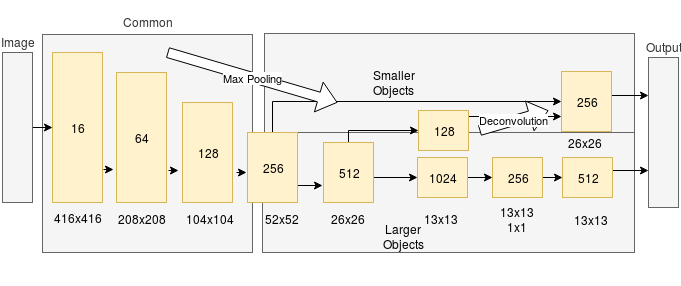
\includegraphics[width=0.8\textwidth]{fig/tinyyolov3_arch}
		\caption{The architecture of the baseline \textit{TinyYoloV3}. For each layer the amount of filters are displayed. The height of the boxes correspond to their spatial dimension. Arrows correspond to the forward pass in a network inference. In the common part the spatial resolution decreases each layer down to 26x26, while the width increases from 16 to 512. From layer 5 two branches focus on objects corresponding to different scales. }
		\label{fig:tinyyolov3_arch}
	\end{figure}
	

	\subsection{Training Goal}
	
	In order to train a \ac{CNN} to predict the desired properties a ground truth has to be defined for each of the 12675 output nodes. Subsequently the loss is formulated as derivable function and the \ac{CNN} can be trained with backpropagation.
	
	Thereby it is desirable that a network output of zero corresponds to no network activation and henceforth to keep all predicted bounding boxes in the default shape. Therefore, \textit{YoloV3} encodes the ground true coordinates as follows:
	 
	
	\begin{equation}
	\label{sec:encoding}
	b_x = \sigma(\hat x_{i,j,k}) + g^x_{i,j}\quad
	b_y = \sigma(\hat y_{i,j,k}) + g^y_{i,j}\quad
	b_w = e^{\hat w_{i,j,k}} \cdot p^w_{i,j,k}\quad
	b_h = e^{\hat h_{i,j,k}} \cdot p^h_{i,j,k}
	\end{equation}
	
	where $\hat{x}$,$\hat{y}$,$\hat w_{i,j,k}$ and $\hat h_{i,j,k}$ correspond to output nodes of anchor box at grid $i$, cell $j$, anchor $k$; $g^x_{i,j,k}$, $g^y_{i,j}$ is the top left coordinate of the respective grid cell; $\sigma$ is the sigmoid-function.
	
	The question remains to which grid cell and anchor box a label is assigned to. Therefore the \ac{IoU} between every ground truth and anchor box is calculated and the grid with the highest value is assigned. If a ground truth box has very different coordinates than any possible anchor box, even the highest \ac{IoU} is comparatively low. Thus the network has to perform a very strong activation to predict such a label. In return the gradient will be high which can cause unstable updates. Therefore labels that have a lower \ac{IoU} than 0.5 are excluded. 
	
	With the true label and the predicted label the training goal can be formulated. The loss needs to capture the localization and the classification goal. In a typical ground truth image only a small subset of anchors is assigned responsible to predict an object. All the other anchors see only background. Hence, there is a class imbalance between the "object" class and the "background" class. Treating both losses equally would lead the model to simply assign "background" for all anchors. The weight terms $\lambda_{obj}$ and $\lambda_{noobj}$ compensate for this class imbalance. Furthermore, $\lambda_{loc}$ trades-off the localization goal and the classification goal. The abstract training loss is summarized in: 

	\begin{equation}
	\mathcal{L} = \lambda_{loc}\mathcal{L}_{loc} + \lambda_{obj}\mathcal{L}_{obj} + \lambda_{noobj}\mathcal{L}_{noobj} + \lambda_{class}\mathcal{L}_{class}
	\end{equation}
	where $\mathcal{L}_{loc}$ is the loss for bounding box dimensions, $\mathcal{L}_{obj}$ the loss where a object is present, $\mathcal{L}_{noobj}$ the loss where there is no object. The weights are kept to the default value of $\lambda_{loc} = 5$,$\lambda_{obj} = 5$ and $\lambda_{noobj} = 0.5$.
	
	The object loss quantifies a binary classification loss. Hence, it is the difference between a predicted probability $\hat o$ and an actual class label $c$. Where $o \in \{0,1\}$ and $\hat o \in (0,1)$. In order to learn such a goal it is desirable that the weights of the network get updated significantly when the difference between truth and prediction are high. However, when prediction and truth are already close to each other, the updates to the weights should be smaller otherwise the training might miss the optimal solution. A loss function that contains the desired properties and is used by \textit{YoloV3} is the logarithmic loss which can be formulated as follows:
	
	\begin{equation}
		\mathcal{L}_{log} = -(o_{ij}\log(\hat o_{ijk}) + (1 - o_{ij})\log(1 - \hat o_{ijk}))
	\end{equation}
	
	where $\hat o_{ij}$ is an output node with sigmoid activation assigned to anchor box $i$,$j$,$k$ and $ o_{ij}$ the ground truth label assigned to that box. The logarithmic loss is calculated for each output grid $G_i$, for each grid cell $S_j$ and each anchor box $B_k$. However, only the loss of the responsible anchor boxes are summed in the total loss calculation:
	
	\begin{equation}
		\mathcal{L}_{obj} = \sum_{i=0}^{G}\sum_{j=0}^{S_i^2}\sum_{k=0}^{B_i} \mathbb{1}_{ijk}^{obj}(-(c_{ijk}\log(\hat c_{ijk}) + (1 - c_{ijk})\log(1 - \hat c_{ijk})))
	\end{equation}
	
	Thereby the  binary variable $\mathbb{1}_{ijk}^{obj}$ is 1 if an object is present at anchor $i,j,k$. $\mathcal{L}_{obj}$ is defined vice versa but controlled by the $\mathbb{1}_{ijk}^{noobj}$ binary variable.

	For the localization loss, similar to the classification loss, the weights should be updated significantly when the difference is high but less strongly when the difference is small. Furthermore, the loss should be invariant to direction. A loss that contains these properties is the squared distance between each bounding box parameter. However, the squared distance does not make a difference between large and small boxes. For example, a deviation of 5 px for a small ground truth box with a width of 1 is treated equally to a deviation from a ground truth box with width 100. Therefore \textit{YoloV3}, applies the square root on width and height to scale down very large box dimensions and thus balance the loss calculation. The localization loss is summarized in:
	
	\begin{equation}
		\mathcal{L}_{loc} = \sum_{i=0}^{G} \sum_{j=0}^{S_i^2}\sum_{k=0}^{B_i} \mathbb{1}_{ijk}^{obj}[(x_{ijk}-\hat{x}_{ijk})^2 + (y_{ijk}-\hat{y}_{ijk})^2  + (\sqrt{w_{ijk}}-\sqrt{\hat{w}_{ijk}})^2 +(\sqrt{h_{ijk}}-\sqrt{\hat{h}_{ijk}})^2 ]
	\end{equation}
	where $x_{ijk}$,$y_{ijk}$ are the ground truth center coordinates of anchor box $i,j,k$ and $w_{ijk}$,$h_{ijk}$ the corresponding width and height. $\hat x_{ijk}$,$\hat y_{ijk}, \hat w_{ijk}$,$\hat h_{ijk}$ are the predicted bounding box coordinates. 
	
	The model is implemented using \textit{keras} with \textit{tensorflow} backend. 
	
	\section{Detecting Empty Objects}
	
	As could be seen in \Cref{sec:methodology}, \textit{TinyYoloV3} similar to most current \acp{CNN} combine simple features to a more abstract representation layer by layer. Thereby pooling reduces task irrelevant information and reduces the spatial dimension. At the same time the number of filters is increased to encode the more complex patterns. In the deeper layers information of larger areas in the image is combined. In the final layer each location in the volume encodes the patterns that are present in the respective field of the preceding filters and an object prediction is performed.
	
	The power of deep \acp{CNN} arises from their capability to learn very complex patterns. However, these are not present in \acp{EWFO}. Instead most of the object area consists of background and should be ignored by the detector. Therefore we hypothesize that a simple network should perform equally well on \acp{EWFO} as a much deeper network. However, for a more complex object the performance should increase with a deeper architecture.
	
	Due to the emptiness of the object a detector can be distracted by the patterns that are visible within the empty part. Hence, we hypothesize that a solid object is simpler to detect than an \acp{EWFO}. If this is true the performance should decrease as the empty part gets bigger. This would mean objects that appear closer to the image are harder to detect. This would be the opposite to solid objects. For example \todoref{object detect tensorflow} report an increase in detection performance with object size on the common Object Detection benchmarks.
	

	\subsection{Experiment}
	
	In order to evaluate our hypothesis we compare the detection of the empty object to similar objects that are solid. This is achieved by using the data generation tool to augment the object with a solid part that contains patterns of different complexity. Examples can be seen in \Cref{fig:cats}. 
	
	\begin{figure}
		\centering
		\begin{minipage}{0.3\textwidth}
		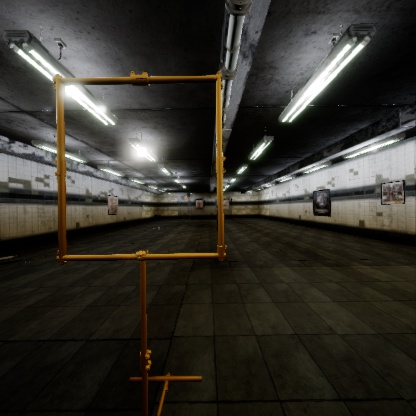
\includegraphics[width=\textwidth]{fig/gate}
		\end{minipage}
		\begin{minipage}{0.3\textwidth}
		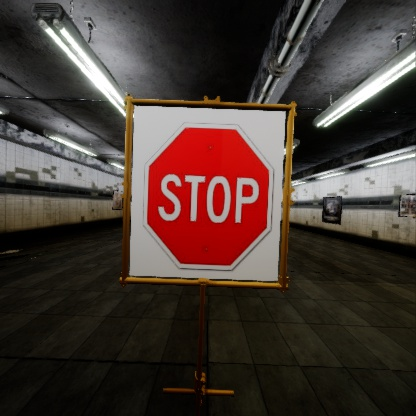
\includegraphics[width=\textwidth]{fig/sign}
		\end{minipage}
		\begin{minipage}{0.3\textwidth}
		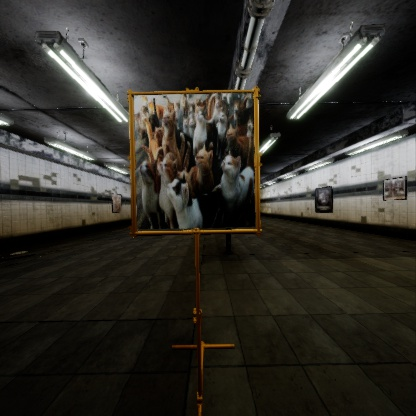
\includegraphics[width=\textwidth]{fig/cats}
		\end{minipage}
		\caption{Examples of the three objects that are compared. The \acp{EWFO} object left is compared to a simple solid object in the center and a complex solid object on the right.}
		\label{fig:cats}
	\end{figure}
	
	For each object a dataset with 20 000 samples is created within the \textit{Basement} environment. On these training sets multiple architectures are trained: 
	
	\begin{itemize}
		\item \textit{TinyYoloV3}: The \textit{TinyYoloV3} architecture serves as baseline for our experiments and is described in fully detail in \Cref{sec:meth}.
		\item \textit{GateNet}: The \textit{GateNet} architecture is based on  \textit{TinyYoloV3}. However, in the initial configuration the network
		\item \textit{Darknet-19}: The \textit{Darknet-19} architecture served as baseline for the \textit{YoloV2} detection network. It takes images of 416x416 as input and processes them the image in 19 layers. The exact architecture can be seen in \todo{text}. For the purpose of object detection we add a prediction layer for small objects at layer 16 and replace the fully connected layer with the prediction layer for larger objects.
	\end{itemize}

	For all trainings the Adam optimizer is applied using a learning rate of 0.001 for the first 60 epochs and a learning rate 0.0001 afterwards. A validation set containing 1\% randomly sampled images from the training set is used. The training is stopped if the validation error does not decrease for more than 5 epochs or 100 epochs are reached.

	Furthermore, test sets are created for each object. Each test set contains 150 samples at various scales. Each architecture is tested on each of the test sets.
	
	
	\subsection{Results}
	
	\begin{figure}
	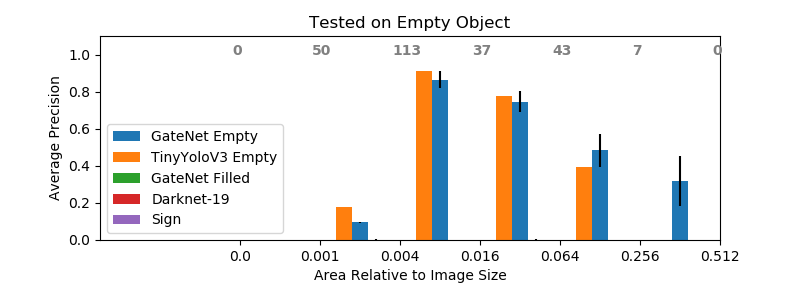
\includegraphics[width=\textwidth]{fig/basement_gate_size}
	\caption{An example of the augmented object. A \acp{CNN} can exploit this structure and should be less distracted by background.}
	\label{fig:basement_gate}
	\end{figure}

	\begin{figure}
	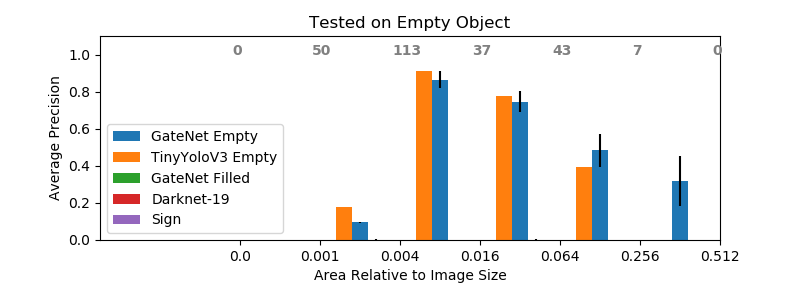
\includegraphics[width=\textwidth]{fig/basement_gate_size}
	\caption{An example of the augmented object. A \acp{CNN} can exploit this structure and should be less distracted by background.}
	\label{fig:basement_sign}
	\end{figure}

	\begin{figure}
	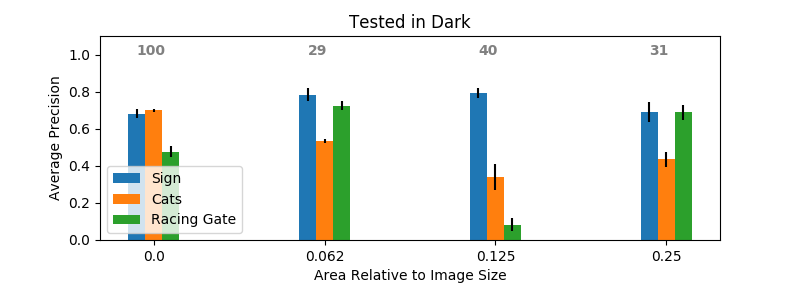
\includegraphics[width=\textwidth]{fig/basement_cats_size}
	\caption{An example of the augmented object. A \acp{CNN} can exploit this structure and should be less distracted by background.}
	\label{fig:basement_cats}
	\end{figure}
	
	\subsection{Discussion}
	
	\subsection{Conclusion}
	
	\section{Creating an efficient architecture}
	
	\begin{figure}[hbtp]
		\centering
		\begin{minipage}{0.3\textwidth}
			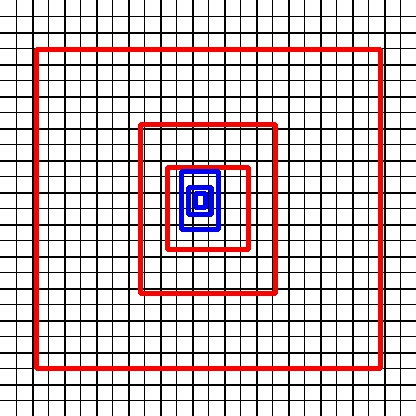
\includegraphics[width=\textwidth]{fig/yolov3_anchors}
		\end{minipage}
		\begin{minipage}{0.3\textwidth}
			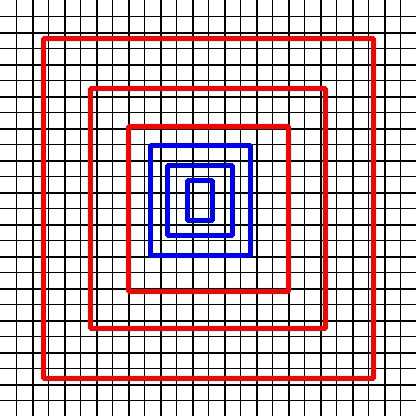
\includegraphics[width=\textwidth]{fig/gate_anchors}
		\end{minipage}
		\caption{ Visualization of the anchor parametrization. It can be seen the two output grids, where the grid for larger scale objects is drawn thicker. For both output grids the anchor at the center location is displayed. The anchor for smaller objects in blue, the anchors for larger objects in red. The left image shows the baseline \textit{TinyYoloV3} anchors. The right image the anchors based on a k-means clustering of the training set. }
		\label{fig:anchors}
	\end{figure}
	
	\textit{TinyYoloV3} is optimized to detect solid feature rich objects of multiple classes with a low computational budget. In order to sufficiently represent and distinguish such objects many weights are required. Hence, the network contains 9 layers and a final width of 1024. In contrast, the features of \acp{EWFO} are relatively simple hence less weights should be required. Therefore we hypothesize a thinner network should be able to learn the task equally well while being computationally more efficient.
	
	The receptive field of \textit{TinyYoloV3} is 223 pixels which does not cover the full input image. For solid objects this is of minor impact as even if the network only sees an object part it can still learn to recognize it. However, this does not apply for \acp{EWFO} which are empty and do not contain any information in the object centre. Instead it can confuse an output layer that is assigned responsible to detect such an object. Therefore we hypothesize that more layers should improve the performance for larger objects. However, the c 
	
	Yet, the complexity of large objects does not increase. Hence, we hypothesize that if the receptive field is large enough,  performance for larger objects. 
	
	Another parameter are network width and depth.  The same condition holds for the number of layers. However, more layers also increase the receptive field. Hence, we expect the performance to increase as long as the receptive field does not fully capture the image.
	
	In order to evaluate our hypothesis we perform an architecture evaluation by varying the number of layers filters and the receptive field. Before training the networks we tune the anchor box dimensions by performing a k-means clustering on t
	

	
	\subsection{Experiments}
	
	Initially an architecture evaluation is performed. Therefore different architectures are trained and evaluated in terms of \ac{ap60}. As an architecture contains many parameters we can not simply vary each of them independently. Hence, three experiments are performed iteratively. We first describe them on a high level basis before explaining the exact changes. In a first step the width is decreased until a drop in performance is noticeable. In a second step the architecture with the lowest width but without performance drop is chosen and the depth is varied. Based on the results of this step we create a final model that combines the gained insights and tune the anchor boxes.
	
	The scheme in which the architecture is changed is visualized in \Cref{fig:depth_changes}. The width of the baseline model is decreased stepwise by a factor of two. When decreasing depth only convolutional layers are removed while the pooling layers are kept such that the spatial resolution stays the same. When increasing depth 2 layers are inserted stepwise at the end of both branches. The results show how depth is mainly relevant to detect objects of larger scale. Hence, the final model consist of 5 common layers, 15 layers on the branch to detect larger objects and 2 layers on the branch to detect small objects.
	
	
	\begin{figure}[hbtp]
		\centering
		\includegraphics[width=0.9\textwidth]{fig/depth_changes}
		\caption{Architectural Changes when varying the depth. The upper graph shows in which order layers are removed. The lower graph shows how layers are added. Depth is increased by inserting two layers on each branch (green). }
		\label{fig:depth_changes}
	\end{figure}
	
	
	
	\subsection{Results}
	
	\Cref{fig:perf_width} shows the performance for thinner and wider networks. It is apparent how the performance only undergoes slight variations despite reducing the total number of weights by a factor 1000. \todo{retrain one in the middle to get variance, it should be more linear}
	
	
	\begin{figure}[hbtp]
		\centering
		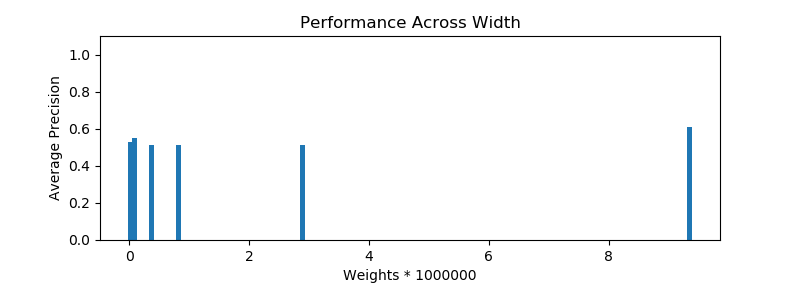
\includegraphics[width=\textwidth]{fig/perf_width}
		\caption{Performance in simulation when varying the amount of filters per layer. Starting from the baseline architecture with approximately 9 Mio. weights, the amount of filters per layer are decreased stepwise by a factor of 2. Only minor effects on performance can be seen, despite reducing the flexibility of the model.}
		\label{fig:perf_width}
	\end{figure}
	
	\begin{figure}[hbtp]
		\centering
		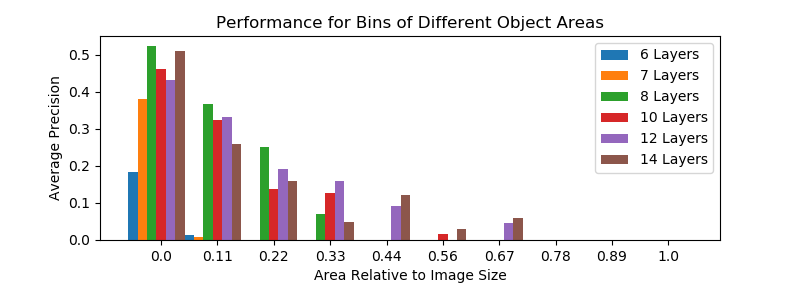
\includegraphics[width=\textwidth]{fig/depth_ap_size}
		\caption{Performance in simulation of models with varying depth and for bins of different size. It can be seen that the performance for larger objects increases with the amount of layers.}
		\label{fig:depth_ap_size}
	\end{figure}
	
	\Cref{fig:size_bins} shows the distribution of object sizes in the bins used for evaluation. It can be seen that most objects in the test set are further away. \todo{put some examples to show what each size actuall means}
	
	\begin{figure}[hbtp]
		\centering
		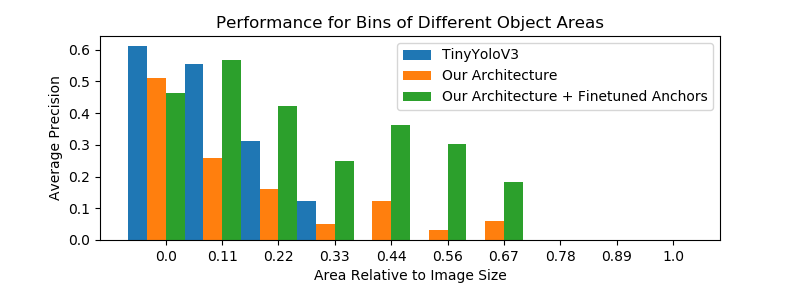
\includegraphics[width=0.8\textwidth]{fig/hyperparam_size}
		\caption{Architectural Changes when varying the depth. The upper graph shows in which order layers are removed. The lower graph shows how layers are added. Depth is increased by inserting two layers on each branch (green). }
		\label{fig:hyp}
	\end{figure}
	
	\begin{figure}[hbtp]
		\centering
		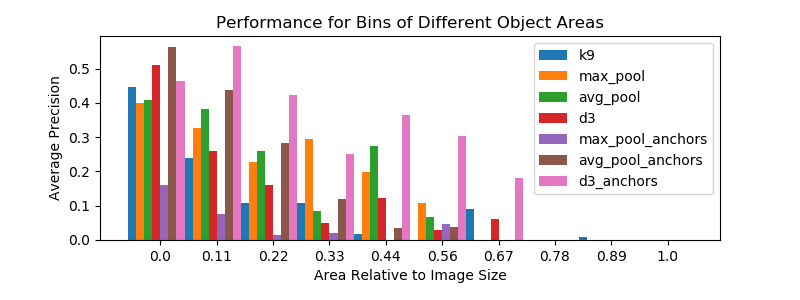
\includegraphics[width=\textwidth]{fig/rf_ap_size}
		\caption{Label distribution in bins of different object size. As the field of view is larger for objects further away, the proportion of small objects is higher.}
		\label{fig:size_bins}
	\end{figure}
	
	\subsection{Discussion}
	
	The overall performance is only slightly affected when reducing the number of weights in terms of width and height. We can assume that this is because the objects we investigate are of quite simple structure. Intuitively the features to be considered are color, lines and edges in certain combinations. Hence, it seems logical that only a few filters are necessary to represent these shapes.
	
	The performance in terms of different object sizes varies significantly for models with varying depth. Only deeper networks are able to detect larger objects. However, the complexity of the object does not increase for closer objects. In contrary the closer the objects are, the less context is visible. A very close object consists "only" of an orange square. Hence, it is unlikely that increased flexibility is the reason for the increase in performance. 
	
	Instead it is more likely that the increased receptive field is the reason for the improved performance. In fact only the network with 14 layers has a receptive field of 414 an thus covers the whole image. Yet even this network cannot detect the largest objects. Thus the receptive field can not be the only reason for the lower performance on larger objects.
	
	The current structure combines features distributed across space in a pyramid fashion. So 3-by-3 convolutions are performed layer by layer such until the whole image is covered. For \acp{EWFO} many of these steps are unnecessary as the objects are empty and the network should learn to ignore the empty part in the centre. It is possible that this structure gets confused by the parts that are present in the image centre.
	
	\subsection{Conclusion}
	
	We investigated how width affects the performance for the detection of \acp{EWFO}. We hypothesized that due to the low variance in the investigated object and the simple features, less filters are required than in the baseline architecture. We can confirm this hypothesis as we see that the width can be decreased by a factor of 10 without loosing performance. This leads to a reduction of weights by a factor of 1000. 
	
	Furthermore, we investigated how depth affects the performance of the model. We hypothesized that a shallow network should be able to detect the object as it only consists of relatively simple features. We can see how depth is required in order to cover the whole input image. Hence, we cannot fully conclude whether depth is required for the increased flexibility or simply due to the receptive field. 
	
	
	\section{Deploying a Detector for \acp{EWFO} on a \ac{MAV}}
	
	
	So far this work investigated the detection of \ac{EWFO} on a theoretical basis. A virtual dataset was created in which different network architectures were evaluated. In this chapter the application of a \ac{CNN} on an example \ac{MAV} is studied. The target system is the JeVois Smart Camera described in \Cref{background:jevois}. The detector is integrated in a control loop that is explained in detail in \Cref{background:system}. The on-board resources give severe limitations to the network that can be deployed. Furthermore, the global state estimation pipeline fuses data from different sensors and over time. Hence, it can be more important to have fast detections that are less accurate compared to slow but accurate detections. Therefore this chapter investigates the performance-accuracy trade-off in the example of the target system. The research question of this chapter is summarized in the following:
	
	\begin{itemize}
		\item[RQ1] What are is the trade-off in terms of accuracy and inference time?
	\end{itemize}
	
	The limited resources on mobile devices makes the deployment of \acp{CNN} a challenging task. For example on pass of the state of the art \ac{CNN} ResNet101 contains of 11.3 billion floating point operations. Even assuming a powerful 2 GHz processor can perform 2 billion calculations per second it would still require almost 6 seconds for one network pass. Furthermore, a \acp{CPU} usually has to reload operands from the memory and cannot directly perform floating point multiplications. Hence, the actual forward pass would require even more time.
	
	Therefore researchers address the reduction of inference time by reducing the number of operations. For example MobileNet and ShuffleNet aim to reduce the computations by addressing the expensive 3D convolutions. Other researchers aim to making the individual operations more efficient. This can be done by replacing floating point operations with integer operations hence quantizing the network.
	
	In order to infer a layer in a \acp{CNN} kernels are convolved at multiple locations within one image. Thereby the same calculations are applied on various input data while the individual operations are independent of each other. Hence, theoretically the computations in one layer can be performed completely in parallel. The output of one layer can be stored similarly to the input image as a matrix. Computational platforms that exploit this fact are \acp{GPU} that have been adopted for Deep Learning applications from early on. In contrast to \acp{CPU} that are optimized to perform many different operations sequentially, \acp{GPU} typically consist of more cores and are optimized to perform the same operation on different data. While each individual core is typically slower than a single core in a \acp{CPU}, \acp{GPU} are much faster for applications that can be performed in parallel.
	
	With a large enough \ac{GPU} it does not matter whether an operation is performed at an image of size 150x150 or 300x300 despite the actual computations increase by a factor of 4. However, such powerful \acp{GPU} require space and energy which is typically not available for small scale \acp{MAV}. The JeVois Smart Camera contains a MALI-400GPU with two cores and 408 Mhz each. Additionally it contains floating point registers and supports NEON operations. These are processor instructions that enable the efficient use of \acp{SIMD} operations.
	
	The actual inference time of a network strongly depends on the computational platform, memory access times as well as the particular low level implementation. Hence, the number of computations within a network can only give a limited insight on the actual inference time. For example the \textit{TensorflowLite} framework allows the deployment of models created in \textit{tensorflow} on mobile processors. However, with this framework a the application of a single kernel on a 104x104 input volume takes 27.1 ms on the JeVois. In contrast, the same operation performed with the \textit{Darknet} framework that supports NEON operations takes only 5.07 ms. 
	
	Therefore, the inference time of several layers is measured on the JeVois using the \textit{Darknet} framework. The results are displayed in \Cref{fig:bottleneck_jevois}. Each sample corresponds to the number of computations and their computational time in one layer. Dashed lines connect samples at the same resolution. It is apparent how the same amount of computations at a spatial resolution of 20x15 is more than 4 times faster than at a resolution of 160x120. 
	
	\begin{figure}[hbtp]
		\centering
		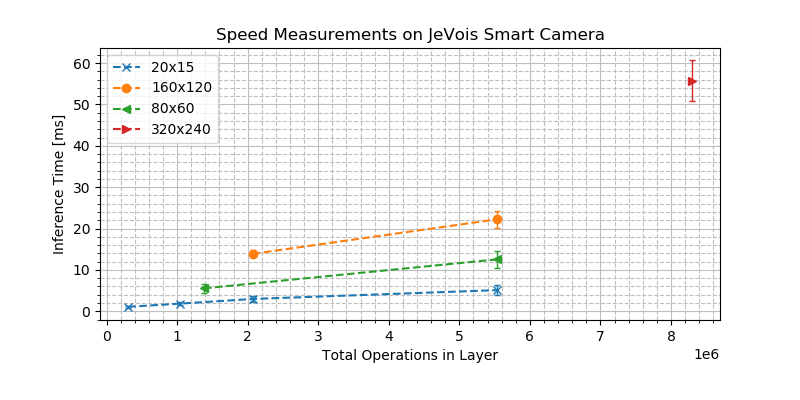
\includegraphics[width=0.8\textwidth]{fig/bottleneck_jevois}
		\caption{Inference Time of different layers on the JeVois. Each sample corresponds to the inference in a single layer. Dashed lines connect samples at the same resolution. It can be seen how an operation at a higher spatial resolution is significantly slower.}
		\label{fig:bottleneck_jevois}
	\end{figure}
	
	Hence, most speed can be gained when reducing the number of computations in the early layers where the spatial resolution is high. In \Cref{sec:object_detection} it could be seen that already a small amount of filters is enough to detect \acp{EWFO}. However, even evaluating 4 kernels at a resolution of 320x240 already takes 55 ms (\Cref{fig:bottleneck_jevois} red triangle). A total network of that size would require more than 200 ms and is thus too slow to be deployed in the control loop. Current research mostly addresses to reduce the computations when the convolved volumes are deep or the operations are performed on \acp{CPU} that do not support floating point operations. However, the bottleneck on the JeVois happens at small volumes and the hardware can perform floating point operations. Furthermore, \acp{EWFO} consist of thin elements that are spread over large parts of the image. Hence, we hypothesize that simply reducing the image resolution will lead to large drops in performance. An alternative is to increase the stride parameter in the early layers of the network. This reduces the number of locations at which the kernel is evaluated. \acp{EWFO} are sparse and spread over large parts of the image, while most of the image does not contain useful information. Hence, we hypothesize that increasing the stride parameter in the early layers will perform better than reducing the image resolution.
	
	\section{Experiments}
	
	In order to evaluate our hypotheses the network is trained with different architectures. Subsequently, performance and inference time on the JeVois are measured.
	
	The JeVois supports aspect ratios of 4:3 and resolutions of 160x120, 320x240 and 640x480. Although, \ac{FCN} do not depend on the image resolution, the object appearance can change at lower image resolution. Hence, during training the images are scaled to 160x160 or 320x320 respectively. The anchor boxes are scaled in similar fashion. Finally, as the input image resolution decreases, the output grid size decreases by the same factor. This is not desirable as the output resolution should stay the same. Hence, when decreasing the input image to 160x160 we remove the last pooling layer such that the output grid stays at 20,20 or 10,10 respectively.
	
	\section{Results}
	
	\begin{figure}[hbtp]
		\centering
		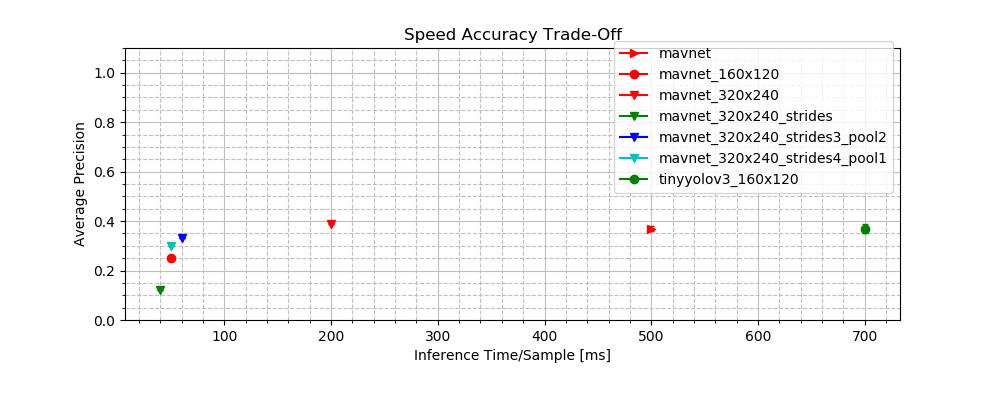
\includegraphics[width=0.8\textwidth]{fig/ap_speed_tradeoff}
		\caption{Inference Time of different layers on the JeVois. Each sample corresponds to a single layer. On the x-axis the total number of multiplications in that layer is displayed. It can be seen how an operation at a higher spatial resolution is significantly slower.}
		\label{fig:ap_speed_tradeoff}
	\end{figure}
	
	Due to their computational complexity deploying a \acp{CNN} on mobile devices is a challenging task
	
	\section{Discussion}
	
	\section{Conclusion}
	
	
	In order to answer this question we measure the inference time of different model architectures. This enables us to investigate the bottlenecks and thus optimize the model architecture. The JeVois Smart Camera uses an aspect ratio of 4:3. Therefore we change the network resolution accordingly. The JeVois Smart Camera has only limited memory available. Using a network architecture that goes beyond the memory simply results in a system crash. For example our baseline network runs performs one network evaluation in 700 ms. This is at a resolution of 160x120.
	

	
	
